\chapter{Propuesta de solución} % Main chapter title
\label{capitulo5} % Change X to a consecutive number; for referencing this chapter elsewhere, use \ref{capitulo5}
Una vez que los requerimientos iniciales han sido fijados y aclarados se busca la manera de automatizar los procesos, investigar tecnologías, y metodologías que ayuden al equipo de desarrollo para entregar funcionalidades de manera iterativa y evolutiva. Durante este proceso se diseñan modelos donde se propone el módulo a ser desarrollado (figura \ref{curriculum_model}) y se busca unir procesos separados del diseño curricular (figura \ref{course_creation_flow}) con el flujo de agregar las competencias, cursos, y programas al AMS (figura \ref{after_creation}).

\begin{figure}[H]
\centering
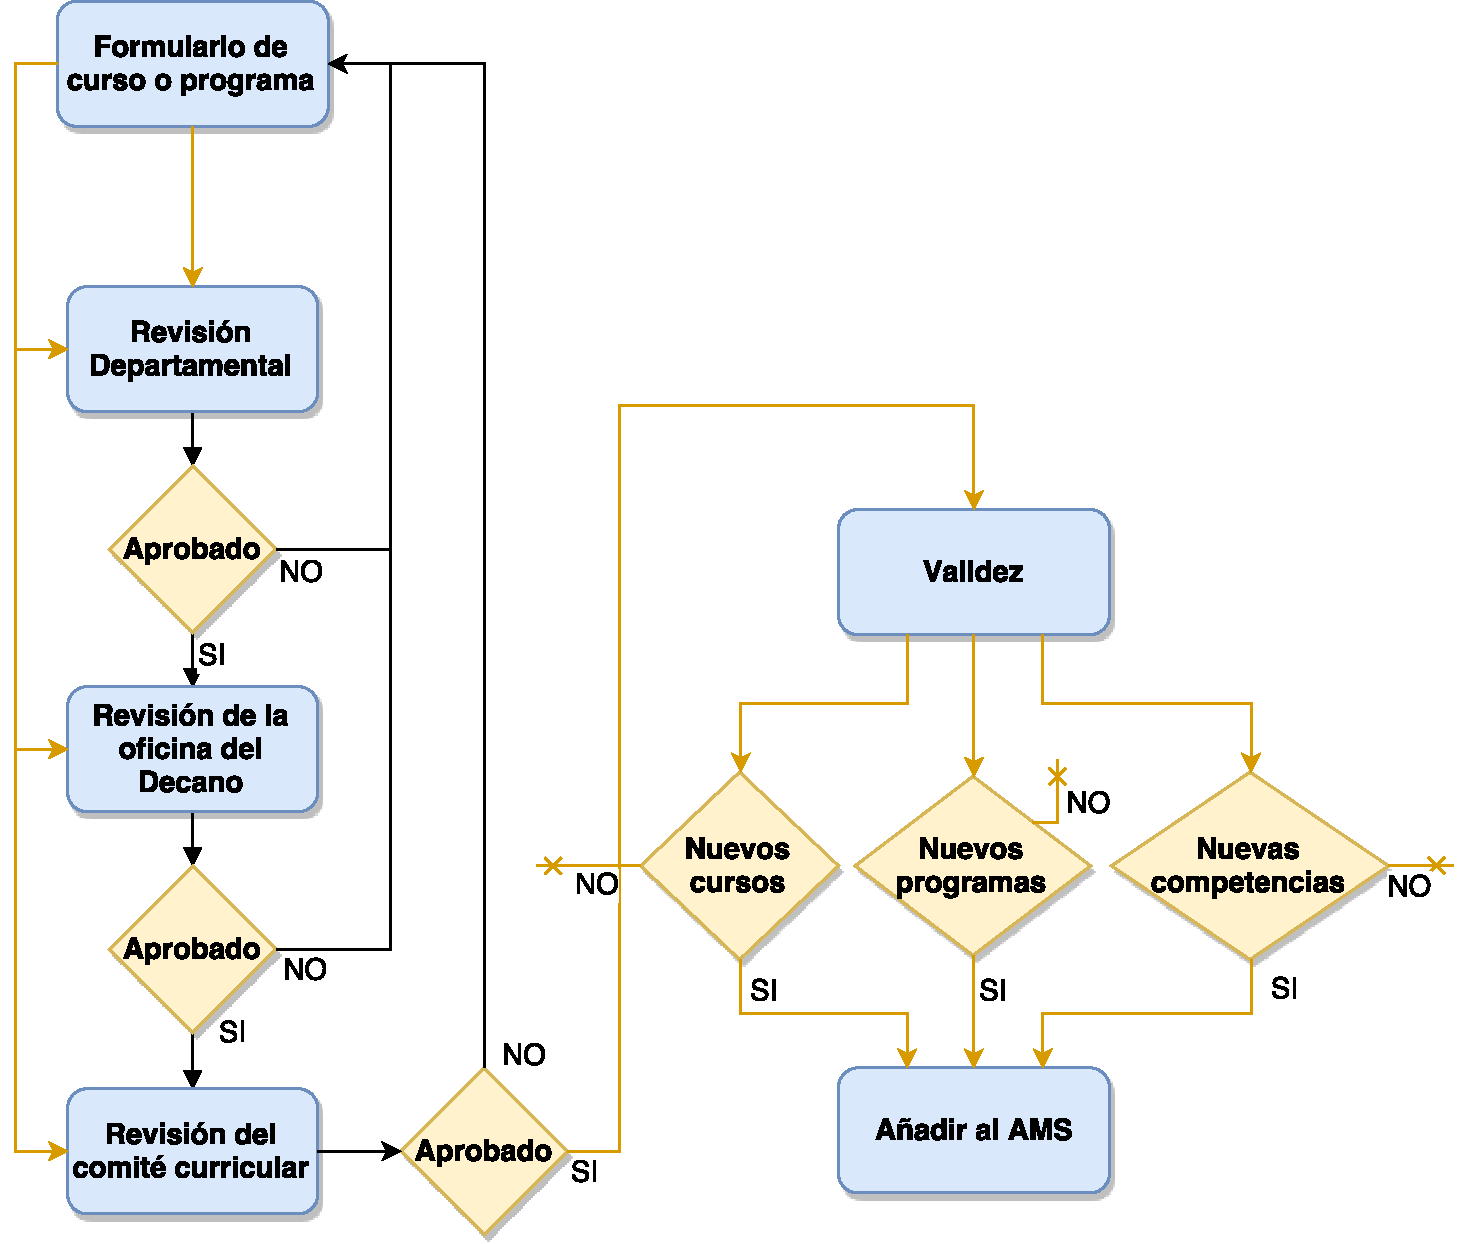
\includegraphics[scale=0.5]{Capitulos/PropuestadeSolucion/Imagenes/curriculum_model}
\caption{Modelo propuesto del módulo curricular adherido a un sistema de gestión de evaluaciones basadas en competencias.}
  \label{curriculum_model}
\end{figure}

Actualmente, cuando el encargado de curso o programa completa su formulario y lo entrega en la mesa de recepción, la misma se encarga de verificar que los datos completados sean válidos y cumpla con el estándar de creación de cursos y programas. 

El módulo propuesto se encargará de automatizar dicho proceso sacando la mesa de recepción como iniciador del flujo de validación mediante un formulario web. Además, se agrega un nuevo tipo de formulario para las competencias de las universidades comunitarias de California.

Luego, pasa por las oficinas del departamento, del decano, y del comité curricular para sus correspondientes revisiones. Si es que una de las oficinas rechaza el formulario debe volver al inicio con el encargado del mismo para volver a ser completado, y una vez terminado puede volver a pasar a la oficina que rechazó el formulario sin necesidad de volver a iniciar todo el proceso de corrección.

Y finalmente, una vez que el comité curricular acepta el formulario se procede a generar los nuevos cursos, programas, o competencias en el AMS. También, otro proceso a ser automatizado por el módulo ya que hoy día dicha creación se hace de manera manual, como se aprecia en la figura \ref{after_creation}.

Se agrega también la funcionalidad de mensajes generados y notificaciones a los integrantes del flujo para evitar de esta manera los cuellos de botella con las revisiones, donde se notifican los pendientes y alertan trabajos en deuda.

\section{Modelo de arquitectura de módulo}

\section{Requerimientos no funcionales} \label{reqnofuncional}
Se ha realizado una breve revisión de las tecnologías y abordajes brindadas como requerimientos funcionales. Sin embargo, al utilizar un abordaje ágil, la validación de las decisiones tecnológicas depende en última instancia de la validación del proceso de desarrollo realizada por expertos y usuarios.

Las decisiones de tecnologías para el módulo de gestión curricular fueron basadas en los conocimientos adquiridos de los miembros del equipo de desarrollo, con el fin de optimizar tiempos utilizados en curvas de aprendizaje. Sin embargo, se hicieron análisis previos a su uso para corroborar que dichas tecnologías cumplen con el propósito de desarrollo.

\subsection{Java}
La elección del lenguaje de programación, establecida por la organización, fue utilizada como lenguaje para la lógica del módulo curricular ya que facilita la integración con el código ya existente. El equipo de desarrollo posee conocimiento en este lenguaje de programación o en lenguajes orientados a objetos, por lo que se aprovechó el tiempo que pudo haber sido utilizado en curvas de aprendizaje del lenguaje para investigar buenas prácticas para el proyecto.

Java fue diseñado para alcanzar los desafíos del desarrollo de aplicaciones en el contexto de ambientes heterogéneos y distribuidos en red \citep{eckel_thinking_2006}. Lo más importante de solucionar entre estos desafíos era la entrega segura de aplicaciones que consumen lo mínimo de recursos del sistema, correr en cualquier plataforma de hardware y/o software, y que pueda ser extendido de manera dinámica \citep{sierra2005head}.

Operar en múltiples plataformas con redes heterogéneas invalida la arquitectura tradicional de distribución de binarios, \enquote{release}, actualización, parcheo, etc \citep{arnold2005java}.

Hoy día, Java es uno de los lenguajes de programación más utilizados a nivel mundial debido a su portabilidad y evolución con el paso del tiempo, como se observa en la Figura \ref{graph_java}. Además, al ser un lenguaje de programación multiplataforma cualquier proyecto se puede desarrollar en cualquier sistema operativo o plataforma para luego ser levantada en el servidor independiente a su plataforma. 

El lenguaje es reconocido por ser intuitivo a la hora de programar, altamente portátil y portable \citep{hunt2011java}. Por otra parte, la comunidad es uno de los fuertes de Java. Además, en la Web hay una gran cantidad de foros y librerías de la comunidad para resolver diferentes problemáticas de los desarrolladores.

\begin{figure}[]
\centering
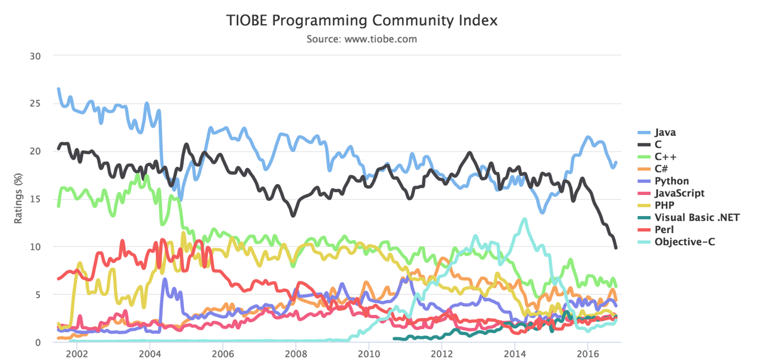
\includegraphics[width=125mm,scale=1]{Figuras/tecnologias/java}
\caption{Gráfico de uso de lenguajes de programación con respecto al tiempo \citep{tiobe_programming}.}
  \label{graph_java}
\end{figure}

El lenguaje Java proporciona un nivel de rendimiento adecuado para la plataforma donde se aloja el AMS.

Dicho uso del lenguaje fue validado durante el proceso de desarrollo al poder resolver los criterios de aceptación de las historias de usuario.

\subsection{MySQL}
Para ayudar a que el AMS sea adaptable y fácil de mantener, se extenderá la base de datos ya utilizada por el AMS. Por lo tanto, la elección de la base de datos del módulo queda a criterio de la organización y como requisito no funcional para el proyecto final. El sistema de base de datos que se utiliza para el sistema de evaluación de competencias es MySQL, por ser un sistema open source y con una de las comunidades más grandes entre las bases de datos existentes.

MySQL es el sistema de base de datos open source más popular disponible. Es particularmente eficaz para sitios web públicos que requieren base de datos rápidas y estables \citep{dyer2015learning}. Para añadir, acceder y procesar datos almacenados en una base de datos informática se necesita de un sistema de administración de Base de Datos como MySQL Server. 

Como las computadoras son muy buenas manejando grandes cantidades de datos, los sistemas de administración de base de datos juegan un rol principal en la computación como utilidades autónomas o como partes de otras aplicaciones.

Para representar los datos que se almacenan, utiliza el modelo lógico de datos relacional donde guarda sus datos en tablas separadas, antes que consolidar todos los datos en un solo lugar. La estructura de la base de datos está organizada en archivos físicos optimizados para mayor velocidad \citep{ronstrom2004mysql}. 

El modelo lógico con objetos tales como bases de datos, tablas, vistas, filas, y columnas, ofrecen un ambiente de programación flexible donde se establecen reglas que gobiernan las relaciones entre las de los distintos tipos de campos, tales como uno a uno, uno a muchos, únicos, requeridos, u opcionales y punteros entre diferentes tablas.

En las siguientes figuras \ref{graph_db_1} y \ref{graph_db_2} podemos observar que MySQL es un sistema de manejo de base de datos muy utilizado por la comunidad y va en aumento de popularidad hasta casi alcanzar a uno de los gigantes que es Oracle.

\begin{figure}[H]
\centering
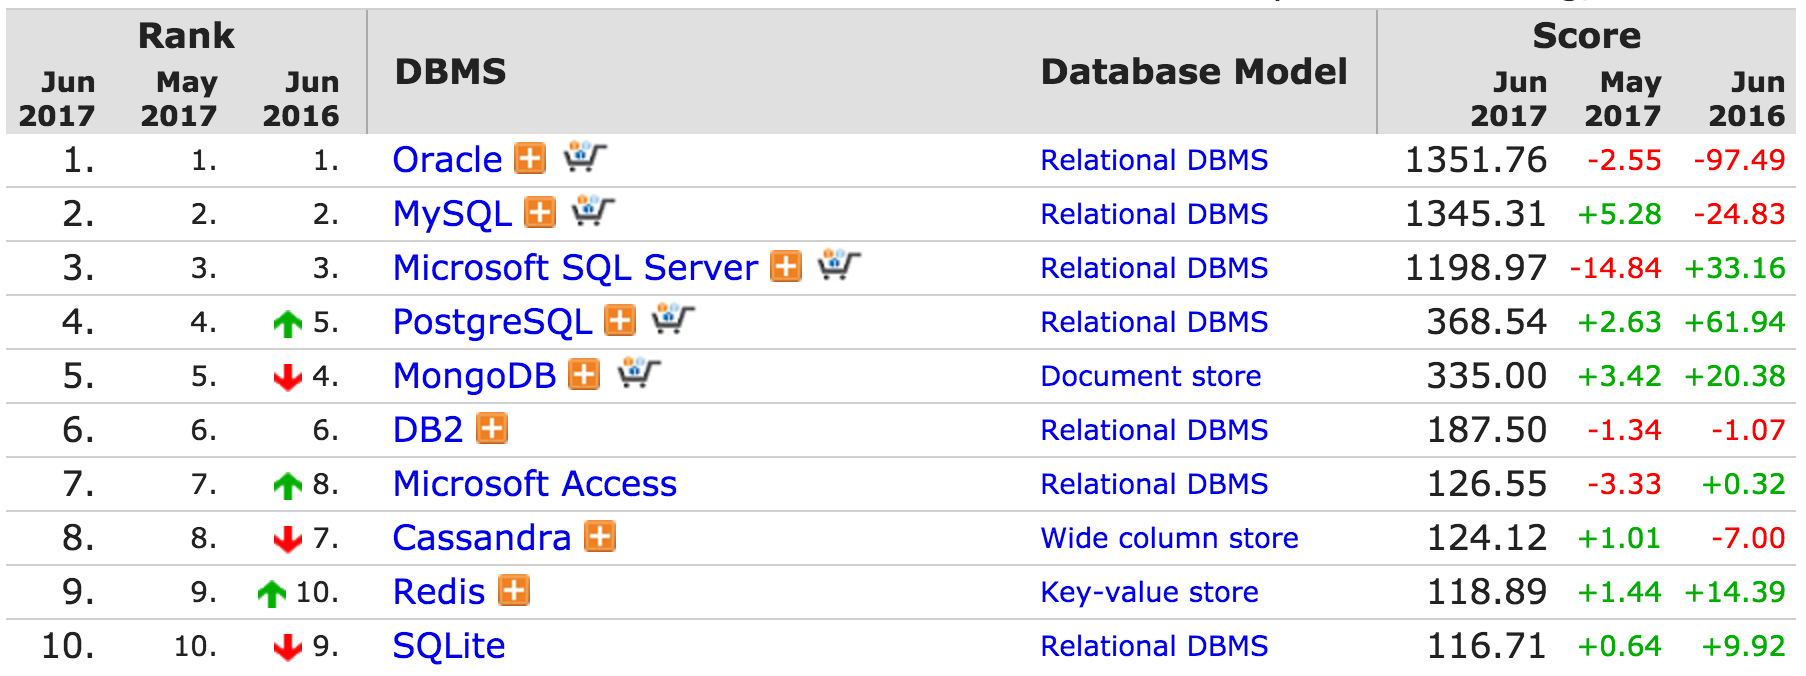
\includegraphics[width=125mm,scale=1]{Figuras/tecnologias/rank_db_1}
\caption{Gráfico que muestra el puntaje de uso de motores de base de datos \citep{db_engines_page}.}
  \label{graph_db_1}
\end{figure}

\begin{figure}[H]
\centering
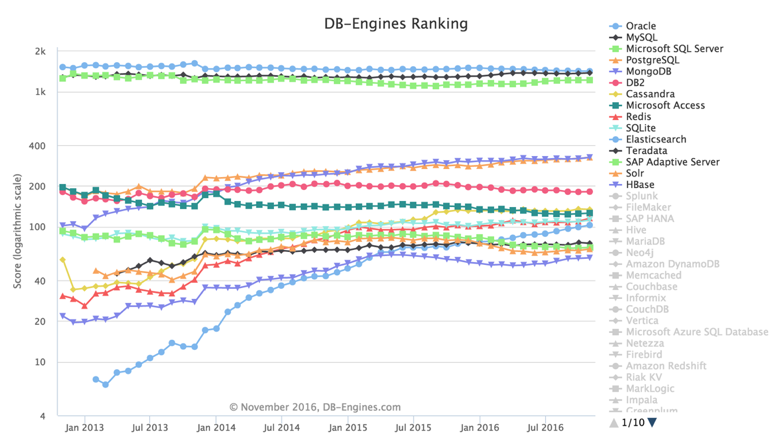
\includegraphics[width=125mm,scale=1]{Figuras/tecnologias/rank_db_2}
\caption{Gráfico de uso de motores de base de datos con respecto al tiempo \citep{db_engines_page}.}
  \label{graph_db_2}
\end{figure}

El motor de base de datos es otro requerimiento no funcional, ya que es otra tecnología utilizada para la aplicación base. Sin embargo, se hizo un breve análisis de vulnerabilidades para verificar que el uso de MySQL como base de datos relacional podría ser efectivo para el proyecto final, además, los desarrolladores están familiarizados con la misma.

\subsection{Amazon Web Services}
Amazon Web Services, o más conocida como AWS, es una plataforma de servicios web que ofrece soluciones de procesado, almacenamiento y redes en diferentes capas de abstracción. Se pueden usar estos servicios para hospedar sitios web, correr aplicaciones complejas y para minería de grandes cantidades de datos \citep{wittig2015amazon}. 

La interfaz web puede ser manejada por máquinas o por usuarios mediante de una interfaz de usuario gráfica. Los servicios más utilizados son EC2 en la cual ofrece servidores virtuales, y S3 que es utilizada para almacenamiento.

AWS es una nube pública, donde tiene las siguientes clasificaciones como nube:
\begin{itemize}
	\item \textbf{Infraestructura como Servicio:} más conocida como IaaS, ofrece recursos fundamentales como procesamiento, almacenamiento, y capacidades de servicios, utilizando servidores virtuales tales como Amazon EC2, Google Compute Engine y Microsoft Azure en las máquinas virtuales.
	\item \textbf{Plataforma como Servicio:} más conocida como PaaS, provee plataformas para desplegar aplicaciones customizadas a la nube, tales como AWS Elastic Beanstalk, Google App Engine, y Heroku.
	\item \textbf{Software como Servicio:} más conocida como SaaS, combina infraestructura y software corriendo en la nube, incluyendo aplicaciones de oficina como Amazon WorkSpaces, Google Apps for Work, y Microsoft Office 365.
\end{itemize}

En la figura \ref{graph_cloud} se puede mostrar como AWS lidera entre las alternativas del mercado para soluciones de computación en la nube. Luego, lo sigue Azure de Microsoft como siguiente alternativa más utilizada. AWS y Azure son líderes en opciones de cloud debido a su constante innovación en el mercado como se puede apreciar en la figura \ref{gartner_cloud}.

\begin{figure}[H]
\centering
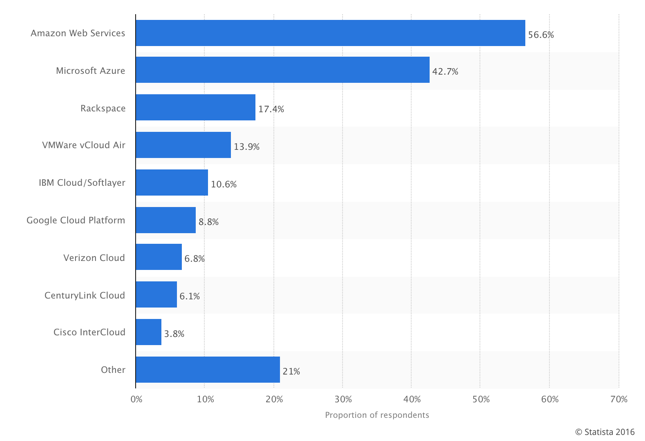
\includegraphics[width=125mm,scale=1]{Capitulos/PropuestadeSolucion/Imagenes/rank_cloud}
\caption{Ranking de compañías que brindan servicios de cloud computing \citep{statista_ranking}.}
  \label{graph_cloud}
\end{figure}

\begin{figure}[H]
\centering
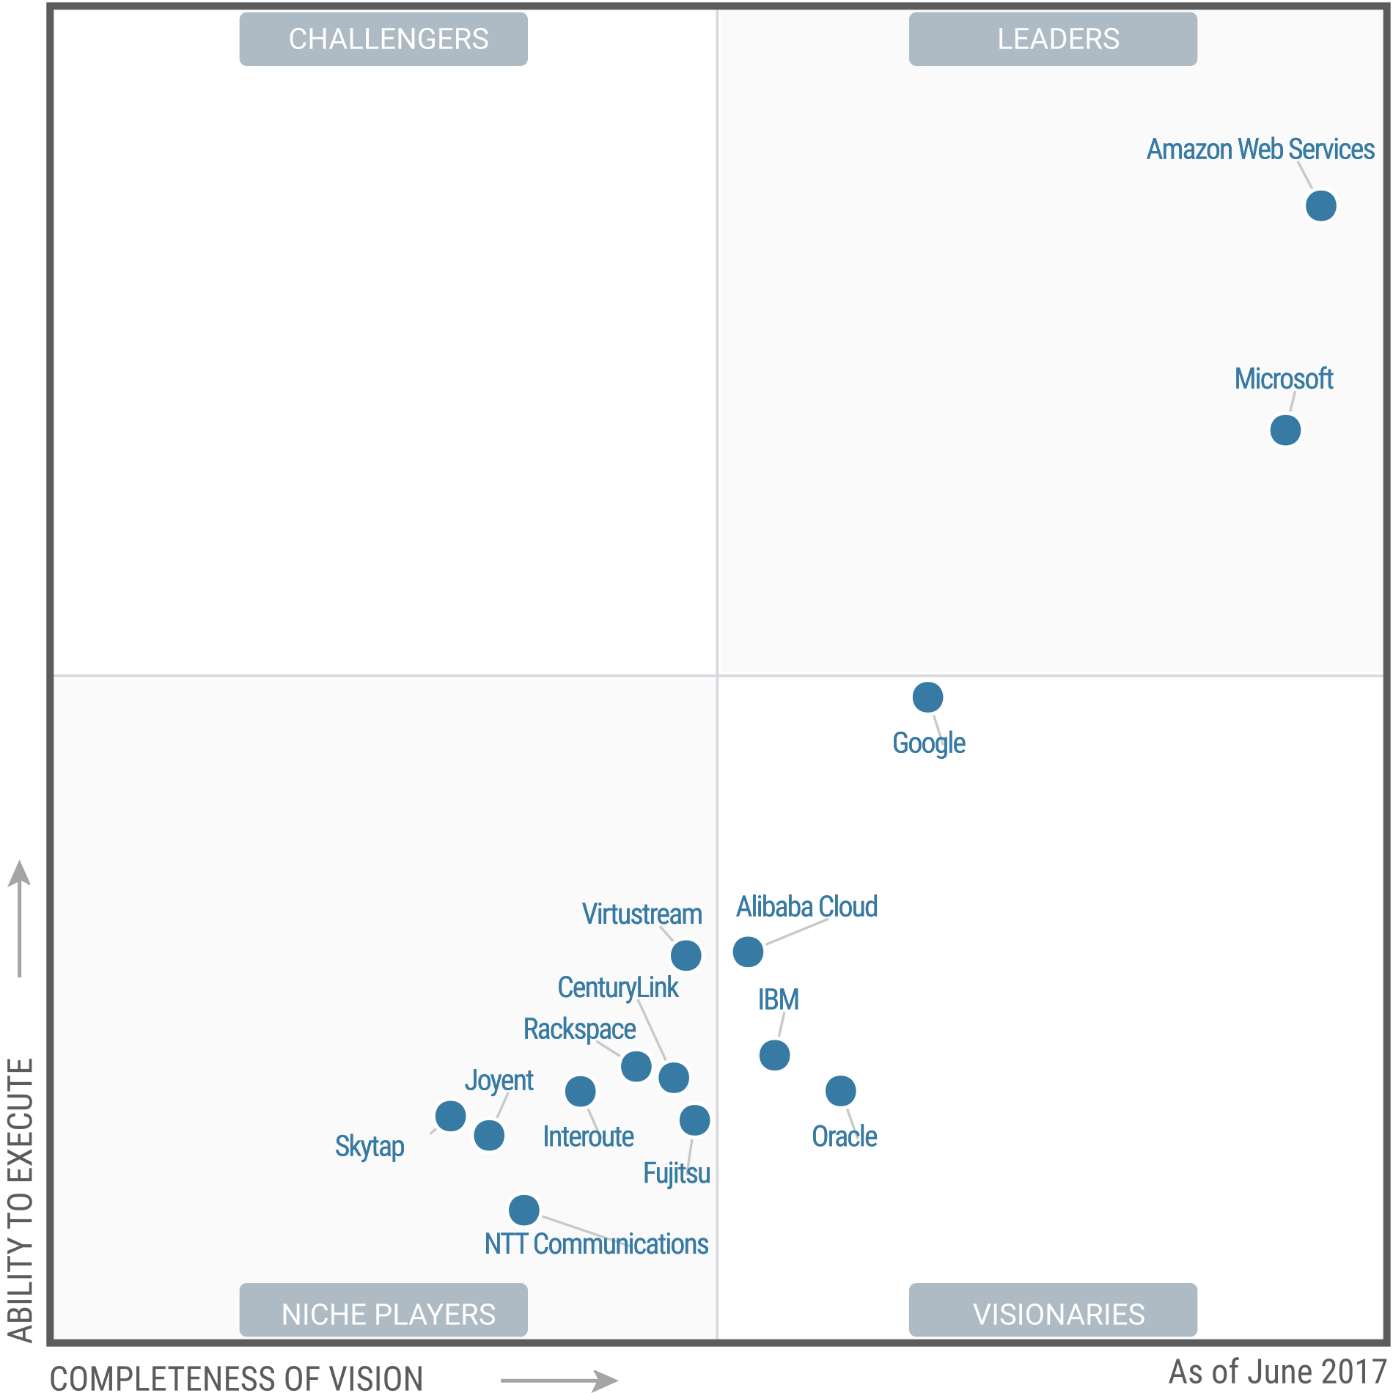
\includegraphics[scale=0.5]{Capitulos/PropuestadeSolucion/Imagenes/gartner_cloud}
\caption{Figura de Gartner que muestra las alternativas de cloud computing \citep{gartner_webpage}.}
  \label{gartner_cloud}
\end{figure}

El AMS se encuentra alojado en la plataforma de servicios AWS. Por lo tanto, se utilizaron los servidores ya en línea para correr el módulo curricular para la aplicación.

\subsection{Git}
Como un equipo de desarrollo requiere de un sistema de control de versiones eficiente, se utilizó Git por ser el líder en VCS \citep{loeliger2012version}. Para mejorar la integración del código que produce el equipo, la organización utiliza un repositorio en \enquote{GitHub}\footnote{Plataforma de desarrollo colaborativo de software para alojar proyectos utilizando el sistema de control de versiones Git.}. Además, el uso de un sistema de versionamiento permite minimizar y optimizar el tiempo de unión de módulos que van agregando o actualizando los miembros del equipo de desarrollo.

El control de versiones es un sistema que registra los cambios realizados sobre un archivo o conjunto de archivos a lo largo del tiempo, de esta forma permite recuperar versiones específicas más adelante \citep{chacon2014pro}.

Git modela sus datos más como un conjunto de instantáneas de un pequeño sistema de archivos. Cada vez que se confirma el cambio de un archivo, o se guarda el estado de un proyecto se hace una foto del aspecto de todos los archivos en ese momento y guarda una referencia a esa instantánea. Para ser eficiente, si los archivos no se han modificado, Git no almacena el archivo de nuevo, solo un enlace al archivo idéntico anterior que ya tiene almacenado. Este comportamiento se puede observar en la figura \ref{graph_git}.

\begin{figure}[H]
\centering
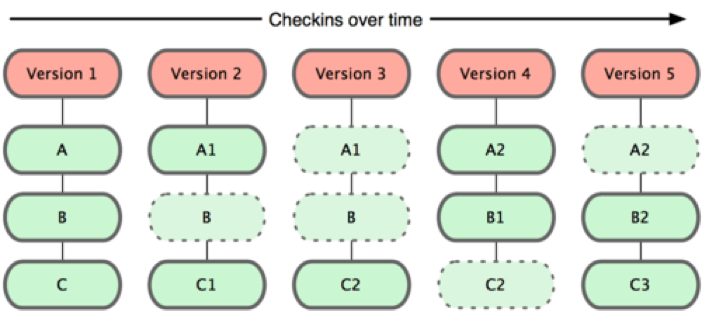
\includegraphics[width=125mm,scale=1]{Figuras/tecnologias/git_over_time}
\caption{Flujo de versiones de Git \citep{chacon2014pro}.}
  \label{graph_git}
\end{figure}

Uno de los fuertes importantes de Git como VCS\footnote{de sus siglas en inglés, Version Control System, que significa en español sistema de control de versionamiento.} es su integridad, debido a que toda versión es verificada mediante una suma de comprobación\footnote{También conocida como checksum.} antes de ser almacenada, y es identificada a partir de ese momento dicha suma. Esta suma es utilizada para volver a un estado anterior del repositorio en caso de ser necesario o ver cuáles fueron los cambios que se realizaron en la porción de código trabajado o más conocido como commit \citep{chacon2014pro}.

\subsection{Spring}
El AMS cuenta con un framework propio desarrollado internamente, el cual esta deprecado y uno nuevo en el cual se estuvo trabajando para los nuevos módulos que se fueron desarrollando. El mismo es Spring MVC y fue utilizado para la parte lógica de la aplicación.

Spring es un framework que facilita el desarrollo de aplicaciones escritas en Java. El propósito de Spring es manejar la infraestructura de las aplicaciones utilizando el método de inversión de control. Es por ello, que el programador se encargará de programar la lógica de negocio usando objetos simples de Java o POJOs (Plain Old Java Objets) y Spring se encargará de añadir las capacidades de empresa o J2EE a la aplicación \citep{bauer2005hibernate}.

Spring tiene las siguientes características:
\begin{itemize}
	\item Simplicidad y acoplamiento débil donde permite programar Java de manera sencilla. Busca ser simple y se basa en la inyección de dependencias para obtener un acoplamiento débil.
	\item Funciona como contenedor ya que gestiona el ciclo de vida de los objetos y como se relacionan entre ellos. Proporciona una gran infraestructura que permite que el programador se dedique a la lógica de la aplicación.
	\item Ligero porque es muy rápido en tiempo de procesamiento y no es invasivo a la hora de programar.
	\item Orientado a aspectos, lo que permite facilitar una capa de servicios que son ideales para este tipo de programación como auditoría, o gestión de transacciones.
\end{itemize} 

Spring se utiliza en el proyecto como framework para toda la aplicación, por lo tanto, usar Spring es también un requerimiento no funcional.

\subsection{AngularJS}
Para empezar a trabajar con la interfaz de usuario se hizo un análisis previo de las ventajas entre Frameworks como JQuery y AngularJS, debido a que la organización que brinda el AMS dio total libertad a la hora de elegir cual utilizar. Por lo tanto, la elección del framework Javascript del módulo de Curriculum entra como decisión de diseño para el proyecto final. 

Con la llegada de los framework de Javascript, tales como JQuery, las páginas web ya no tenían la necesidad de volver a renderizar las páginas cada vez que se necesitaba información del servidor, ya que con la aparición de las llamadas asíncronas se ha logrado mejorar la experiencia del usuario \citep{ruebbelke2015angularjs}.

JQuery ha hecho un excepcional trabajo al proveer de herramientas que manipulen el DOM de una página, pero no ofrece una guía real de cómo organizar el código en la estructura de la aplicación. Ante la desesperada búsqueda de escribir aplicaciones grandes y fáciles de mantener en Javascript ha dado a luz a un renacimiento de frameworks de Javascript, entre ellos se encuentra el framework de Google más conocida como AngularJS.

AngularJS es un framework de aplicaciones web de código abierto que ofrece a un desarrollador una base estable de código con una comunidad enorme y un entorno rico de librerías hechas por la comunidad \citep{darwin2013angularjs}.
\section{Proceso de desarrollo}
El módulo como proyecto de desarrollo enfocado a la metodología Ágil se encuentra dividido en varias épicas para partir en las funcionalidades.

Una épica se encuentra dividida en varias historias de usuario (Figura \ref{epic}), donde las historias de usuario tienen el propósito de entregar valores de negocio al cliente en un periodo establecido de 2 semanas como sprint. Estas historias de usuario pueden ser a la vez divididas buscando la simplicidad de las historias donde cada una debe seguir la práctica INVEST de la metodología Ágil.

Cada historia puede estar compuesta de tareas que tienen como propósito servir al desarrollador como recordatorio de algunas labores pendientes a la hora de desarrollar la historia. Cada tarea debía tener un encargado, pero eso no significaba que esa persona debía hacer sola la implementación.

\begin{figure}[H]
\centering
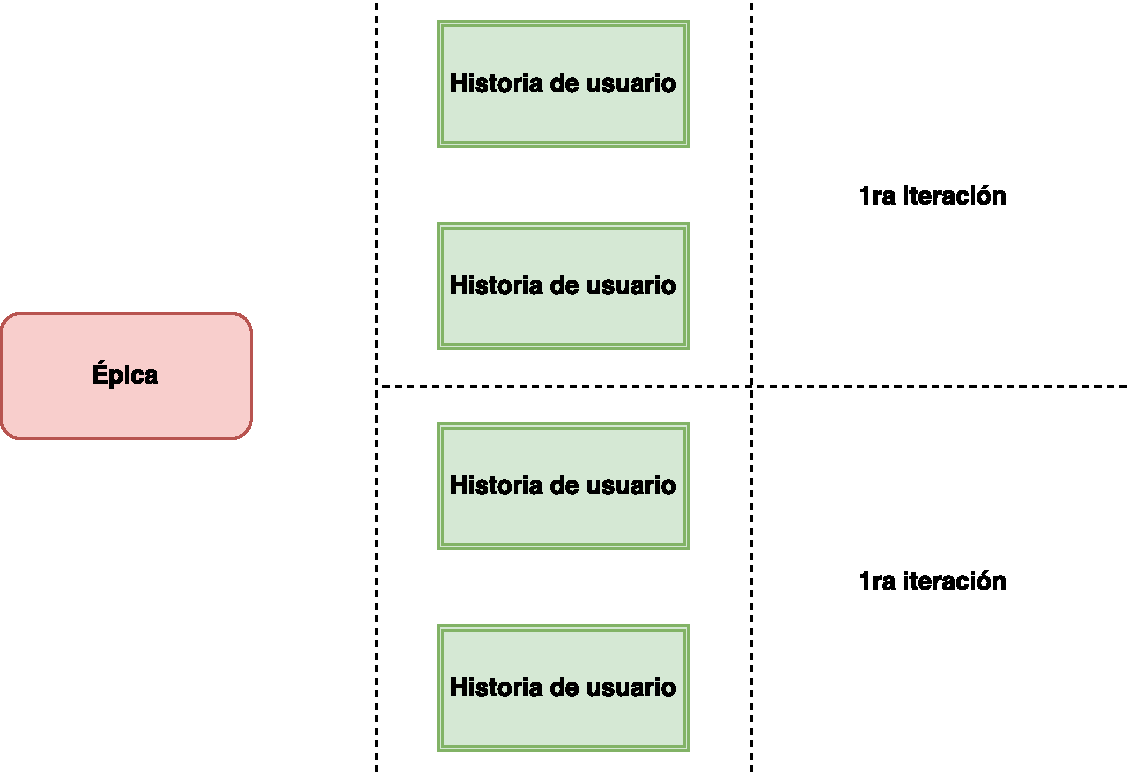
\includegraphics[width=125mm,scale=1]{Capitulos/PropuestadeSolucion/Imagenes/epic_diagram}
\caption{Diagrama de definición de épicas en la metodología ágil}
  \label{epic}
\end{figure}

El PO\footnote{de sus siglas en inglés, Product Owner, que significa en español dueño del producto.} se encarga de la creación de épicas e historias de usuario, en caso de que la historia sea muy grande para terminar en un solo sprint o iteración se vuelve a partir en historias más pequeñas. 

En el caso de estudio, cada sprint consta de 2 semanas de trabajo, donde los desarrolladores como equipo se comprometen a entregar cierto valor de negocio que ellos estiman poder terminar en dicho periodo. Sin embargo, en caso de que el equipo considere que la totalidad de historias no podrán ser entregadas antes de que termine el periodo se pasa al siguiente sprint o se achica la historia minimizando los criterios de aceptación y los restantes se agregan en otra historia de usuario para las siguientes iteraciones.

Cada equipo tiene un líder, donde cada líder tiene como rol ser la brecha que une al PO con los desarrolladores. El PO se reúne con el líder de cada equipo para verificar las prioridades de las historias de usuario que están pendientes en el backlog\footnote{Bolsa de historias de usuarios pendientes.}. 

Al inicio del diseño de la aplicación se llevará a cabo una serie de diseños de funcionalidad y usabilidad que llevar a la mejor experiencia de uso del módulo de gestión curricular, donde dichos diseños serán validados por el equipo en los Estados Unidos antes de iniciar el desarrollo.

\subsection{Scrum}
Scrum es un proceso en el que se aplican de manera regular un conjunto de prácticas para trabajar colaborativamente, en equipo, y obtener el mejor resultado posible de un proyecto. Estas prácticas se apoyan unas a otras y su selección tiene origen en un estudio de la manera de trabajar de varios equipos altamente productivos.

En Scrum se realizan entregas parciales y regulares del producto final, priorizadas por el beneficio que aportan al PO. Por ello, Scrum está especialmente indicado para proyectos en entornos complejos donde se necesita obtener resultados con el mínimo esfuerzo y los requisitos son cambiantes o poco definidos. Además, en dichos ambientes la innovación, la competitividad, la flexibilidad, y la productividad son fundamentales.

Scrum también se utiliza para resolver situaciones en que no se está entregando al cliente lo que necesita, cuando las entregas se alargan demasiado, los costes se disparan o la calidad no es aceptable, cuando se necesita capacidad de reacción ante la competencia, cuando la moral de los equipos es baja y la rotación alta, cuando es necesario identificar y solucionar ineficiencias sistemáticamente o cuando se quiere trabajar utilizando un proceso especializado en el desarrollo de producto. 

\subsection{Proceso}
En Scrum un proyecto se ejecuta en bloques temporales cortos y fijos que los conocemos como sprints o iteraciones. Estas iteraciones por lo general duran 2 semanas aunque en algunos equipos son de 3 y hasta 4 semanas, límite máximo de feedback y reflexión\citep{davis_agile_2015}. Cada iteración tiene que proporcionar un resultado completo, un incremento de producto final que sea susceptible de ser entregado con el mínimo esfuerzo al cliente cuando lo solicite.

El proceso parte de la lista de objetivos o requisitos priorizada del producto, que actúa como plan del proyecto. En esta lista el cliente prioriza los objetivos balanceando el valor que le aportan respecto a su coste y quedan repartidos en sprints y entregas.

\begin{figure}[H]
\centering
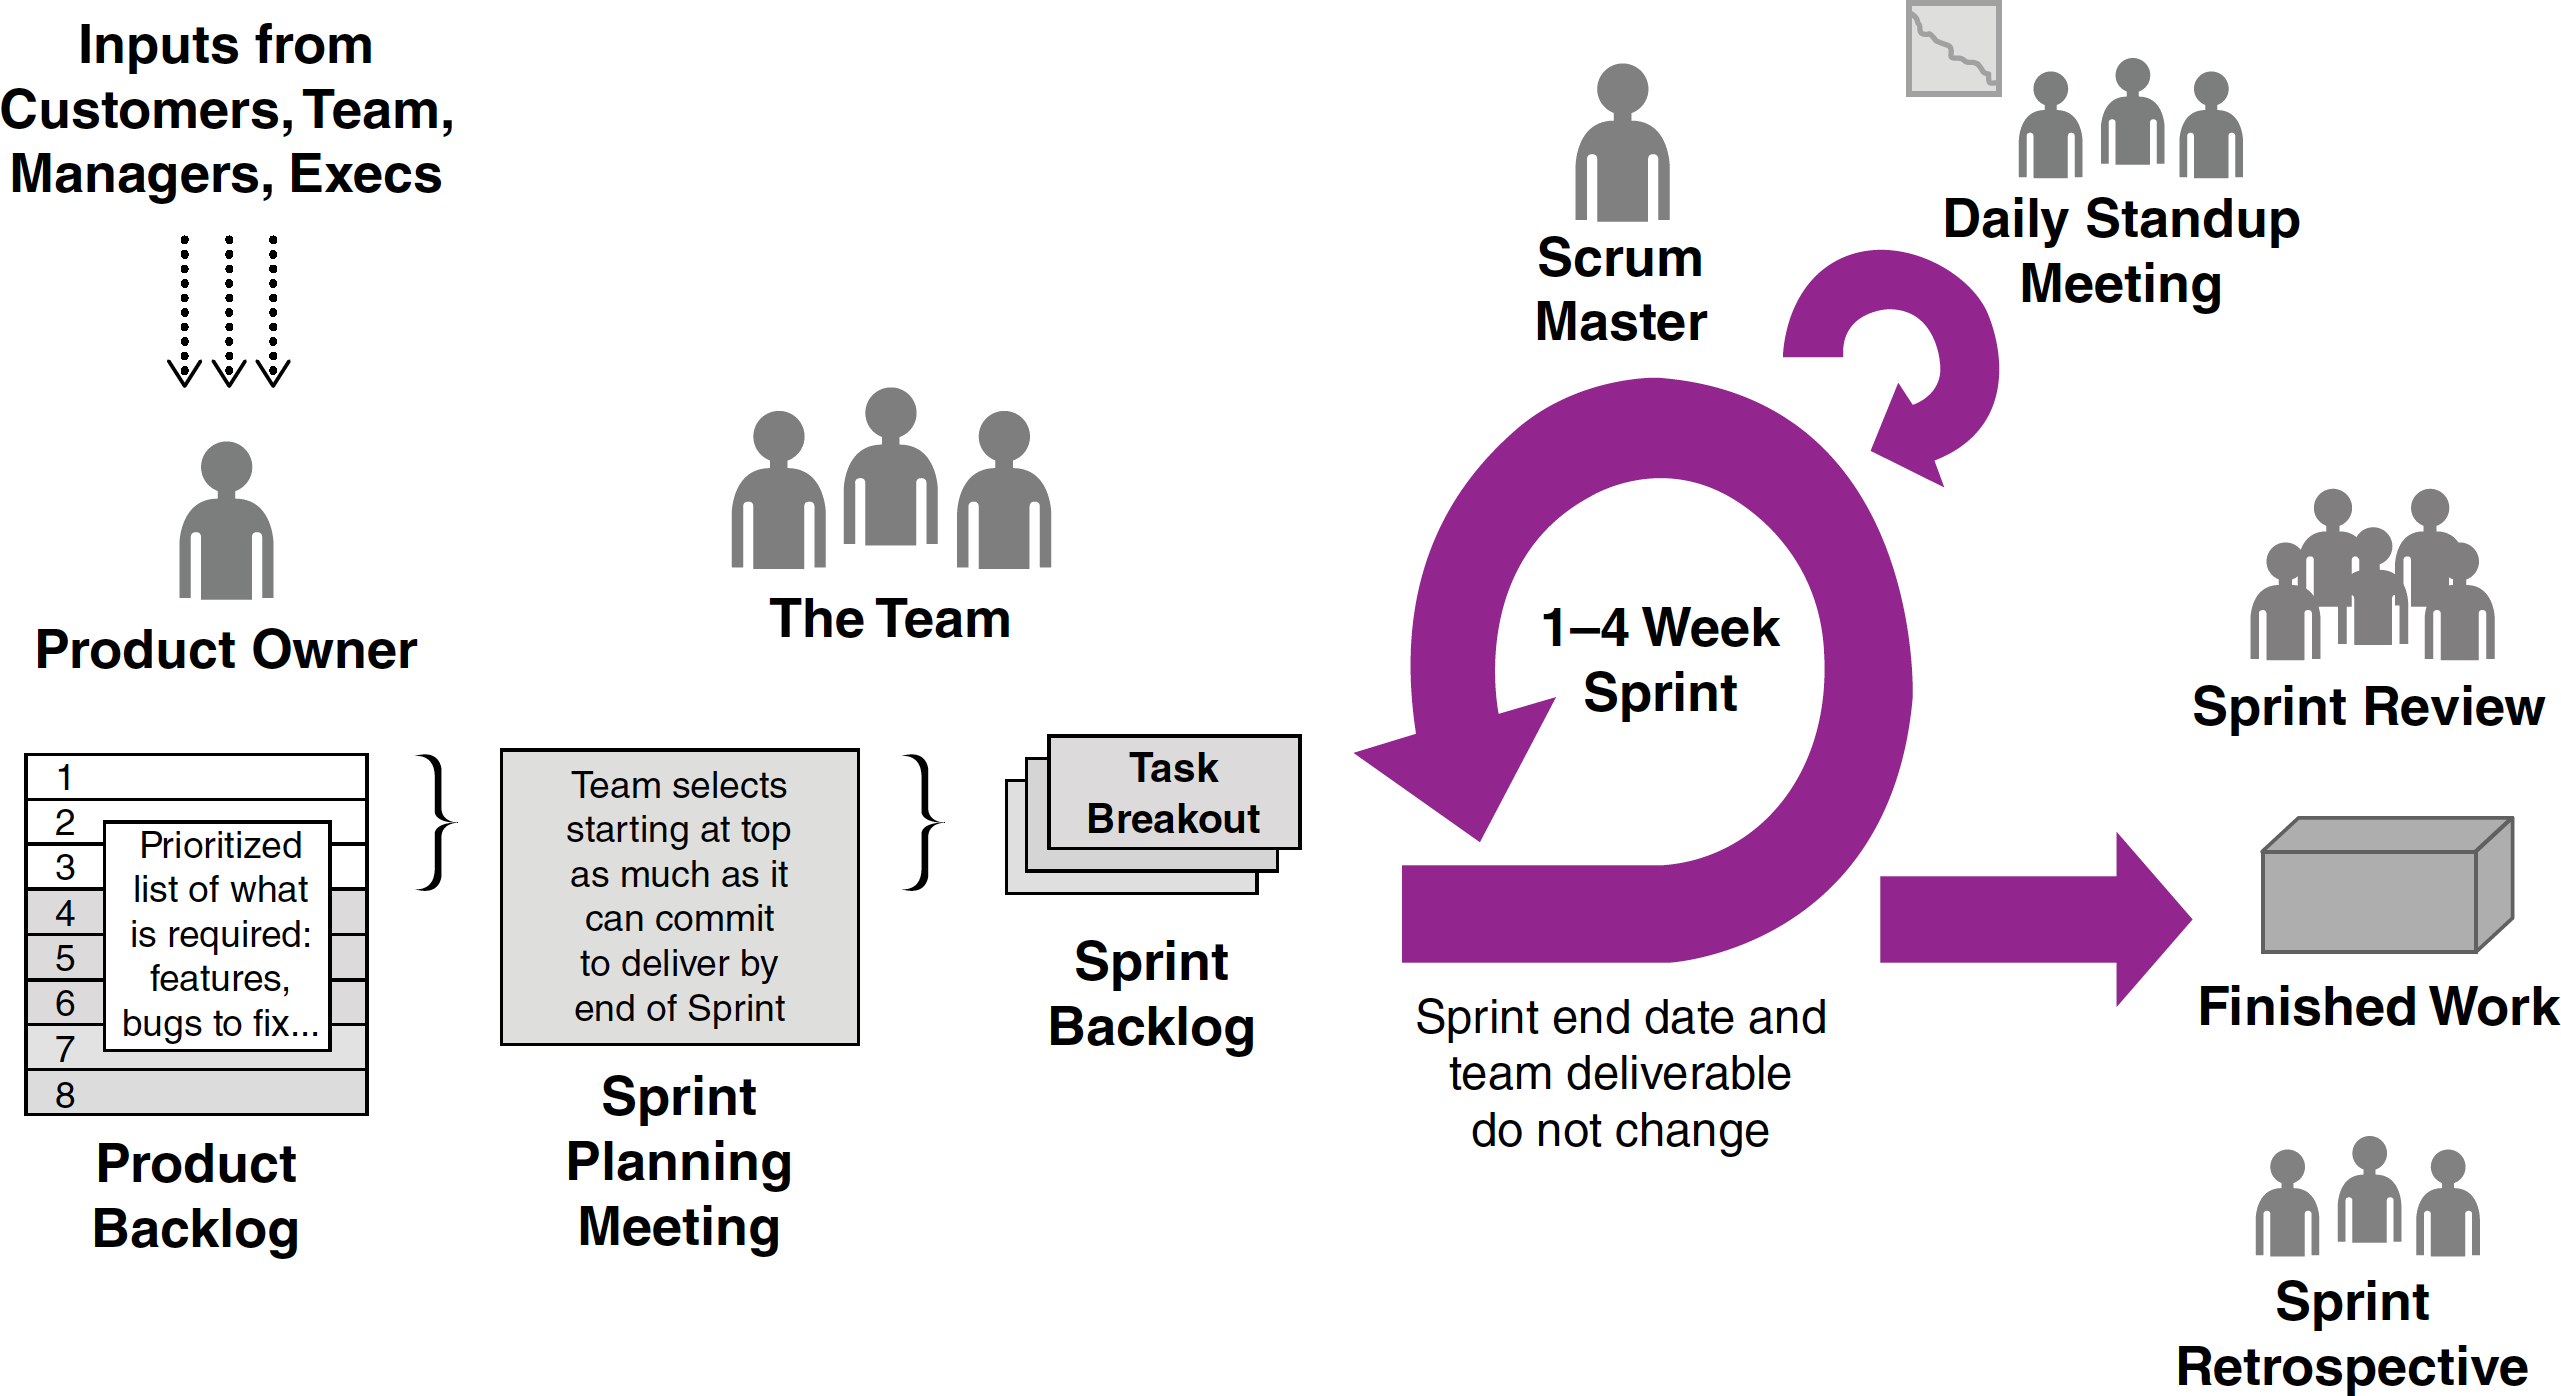
\includegraphics[width=125mm,scale=1]{Figuras/flujo_scrum}
\caption{Flujo de la técnica SCRUM\citep{cobb2015project}.}
  \label{flujo_scrum}
\end{figure}

\subsection{Planificación de iteraciones}
El primer día de la iteración se realiza la reunión de planificación de la iteración y consta de dos partes:
\begin{itemize}
    \item \textbf{Selección de requisitos} (4 horas máximo) – El PO presenta al equipo la lista de requisitos priorizada del producto o proyecto. El equipo pregunta al PO las dudas que surgen y selecciona los requisitos prioritarios que se compromete a completar en la iteración, de manera que puedan ser entregados en caso de ser solicitados.
    \item \textbf{Planificación de la iteración o sprint} (4 horas máximo) – El equipo elabora la lista de tareas de la iteración necesarias para desarrollar los requisitos a que se ha comprometido. La estimación de esfuerzo se hace de manera conjunta y los miembros del equipo se asignan las tareas.
\end{itemize}

\subsection{Ejecución del Sprint}
El equipo realiza una reunión diaria (15 minutos aproximadamente). Cada miembro del equipo inspecciona el trabajo que el resto está realizando (dependencias entre tareas, progreso hacia el objetivo de la iteración, obstáculos que pueden impedir este objetivo) para poder hacer las adaptaciones necesarias que permitan cumplir con el compromiso adquirido. En la reunión cada miembro del equipo responde a tres preguntas:
\begin{itemize}
    \item ¿Qué he hecho desde la última reunión diaria?
    \item ¿Qué voy a hacer a partir de este momento?
    \item ¿Qué impedimentos tengo o voy a tener?
\end{itemize}
Durante la iteración el Scrum Master se encarga de que el equipo pueda cumplir con su compromiso y de que no se merme la productividad del equipo. Además, elimina los obstáculos que el equipo no puede resolver por sí mismo.

Durante el sprint, el PO junto con el equipo refinen la lista de requisitos para prepararlos para los siguientes sprints y, si es necesario, cambian o vuelven a planificar los objetivos del proyecto para maximizar la utilidad de lo que se desarrolla y el retorno de inversión.

\subsection{Inspección y adaptación}
El último día de la iteración se realiza la reunión de revisión del sprint la cual consta de dos partes:
\begin{itemize}
    \item \textbf{Demostración} (3 horas aproximadamente) – El equipo presenta al PO los requisitos completados en la iteración, en forma de incremento de producto preparado para ser entregado con el mínimo esfuerzo. En función de los resultados mostrados y de los cambios ocurridos en el contexto del proyecto, el PO realiza las adaptaciones necesarias de manera objetiva, ya desde la primera iteración, volviendo a planificar el proyecto.
    \item \textbf{Retrospectiva} (1 hora) - El equipo analiza cómo ha sido su manera de trabajar y cuáles son los problemas que podrían impedirle progresar adecuadamente, mejorando de manera continua su productividad. El Scrum Master se encargará de ir eliminando los obstáculos identificados.
\end{itemize}